% ============================================================
%  Mohammad Vazir Panah, Industry CV: Embedded Systems / FPGA
%  Compile with: pdflatex (run twice for the header)
% ============================================================

\documentclass[10pt, a4paper]{article}

\usepackage[T1]{fontenc}
\usepackage[utf8]{inputenc}
\usepackage{microtype}
\usepackage{helvet}
\renewcommand{\familydefault}{\sfdefault}

\usepackage[top=1.6cm, bottom=1.4cm, left=1.8cm, right=1.8cm]{geometry}

\usepackage[table]{xcolor}
\definecolor{navy}{HTML}{1C3557}
\definecolor{accent}{HTML}{2563A8}
\definecolor{midtext}{HTML}{4A5568}
\definecolor{lightbg}{HTML}{EEF2F7}
\definecolor{hdrbg}{HTML}{DDE8F5}
\definecolor{rulecol}{HTML}{CBD5E0}

\usepackage[colorlinks=true, urlcolor=accent, linkcolor=accent,
  pdftitle={Mohammad Vazir Panah CV Embedded}, pdfauthor={Mohammad Vazir Panah}]{hyperref}
\urlstyle{same}

\usepackage{graphicx}
\usepackage{tikz}
\usetikzlibrary{calc}
\usepackage{tabularx}
\usepackage{array}

\usepackage{enumitem}
\setlist[itemize]{leftmargin=1.3em, itemsep=0.5pt, topsep=1.8pt, parsep=0pt, label=\textbullet}

\setlength{\parindent}{0pt}
\setlength{\parskip}{0pt}
\emergencystretch=1em
\hyphenpenalty=10000
\exhyphenpenalty=10000

\usepackage{titlesec}
\titleformat{\section}[block]
  {\normalfont\bfseries\fontsize{10}{13}\selectfont\color{navy}}
  {}{0pt}
  {\tikz[baseline=1.5pt,inner sep=0pt]{\fill[accent](0,0)rectangle(3pt,10pt);}\hspace{6pt}}
  [\vspace{-9pt}{\color{rulecol}\rule{\linewidth}{0.5pt}}]
\titlespacing*{\section}{0pt}{9pt}{4pt}

\usepackage{fancyhdr}
\pagestyle{fancy}
\fancyhf{}
\renewcommand{\headrulewidth}{0pt}
\fancyfoot[C]{%
  \begin{tikzpicture}[remember picture,overlay]
    \fill[navy](current page.south west) rectangle($(current page.south east)+(0,3pt)$);
  \end{tikzpicture}%
  \textcolor{midtext}{\scriptsize Page \thepage}}
\setlength{\footskip}{20pt}

\usepackage{eso-pic}
\newlength{\hdrH} \setlength{\hdrH}{3.9cm}
\newlength{\padX} \setlength{\padX}{1.8cm}
\newlength{\photoD} \setlength{\photoD}{2.75cm}

\AddToShipoutPictureFG*{%
  \begin{tikzpicture}[remember picture, overlay]
    \fill[hdrbg] (current page.north west) rectangle ($(current page.north east)+(0,-\hdrH)$);
    \fill[navy] (current page.north west) rectangle ($(current page.north east)+(0,-4pt)$);
    \draw[navy, line width=1.8pt]
      ($(current page.north west)+(0,-\hdrH)$) -- ($(current page.north east)+(0,-\hdrH)$);
    \begin{scope}
      \clip ($(current page.north east)+(-\padX-\photoD/2,-\hdrH/2)$) circle(\photoD/2);
      \node at ($(current page.north east)+(-\padX-\photoD/2,-\hdrH/2)$)
        {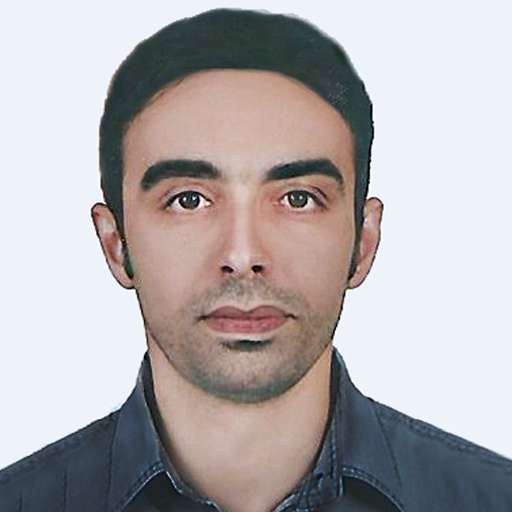
\includegraphics[width=\photoD]{profile.png}};
    \end{scope}
    \draw[white, line width=1.8pt]
      ($(current page.north east)+(-\padX-\photoD/2,-\hdrH/2)$) circle(\photoD/2);
    \node[anchor=north west, inner sep=10pt, text width=\dimexpr\paperwidth-2\padX-\photoD-0.7cm\relax]
      at ($(current page.north west)+(\padX,-4pt-0.16cm)$) {%
      \normalfont
      {\fontsize{22}{26}\selectfont\bfseries\color{navy} Mohammad Vazir Panah}\\[3pt]
      {\fontsize{10}{13}\selectfont\itshape\color{accent}
        Embedded Systems Engineer \,\textperiodcentered\, Embedded Linux, RISC-V, FPGA, C/C++}\\[5pt]
      {\color{rulecol}\rule{\linewidth}{0.4pt}}\\[5pt]
      {\fontsize{8.8}{13}\selectfont\color{midtext}
        Fisciano (SA), Italy
        \,\textperiodcentered\, Permitted to work in Italy
        \,\textperiodcentered\, \href{tel:+393896646511}{(+39) 389\,664\,6511}}\\[3pt]
      {\fontsize{8.8}{13}\selectfont\color{accent}
        \href{mailto:mohammad.vazirpanah@gmail.com}{mohammad.vazirpanah@gmail.com}
        \,\textperiodcentered\, \href{https://www.linkedin.com/in/mohammadvazirpanah}{LinkedIn}
        \,\textperiodcentered\, \href{https://github.com/mohammadvazirpanah}{GitHub}
        \,\textperiodcentered\, \href{https://mohammadvazirpanah.github.io/}{Website}}%
    };
  \end{tikzpicture}}

\newcommand{\IfNonEmptyTF}[3]{\if\relax\detokenize{#1}\relax #3\else #2\fi}
\newcommand{\cventry}[4]{%
  \IfNonEmptyTF{#1}{%
    \begin{tabularx}{\linewidth}{@{}>{\raggedright\arraybackslash}X >{\raggedleft\arraybackslash}p{3.15cm}@{}}
      \textbf{#2} & {\itshape\small\textcolor{accent}{#1}} \\
    \end{tabularx}\par}{\textbf{#2}\par}%
  \IfNonEmptyTF{#3}{\vspace{1pt}{\itshape\textcolor{midtext}{#3}}\par}{}%
  \IfNonEmptyTF{#4}{\vspace{2pt}\begin{itemize}#4\end{itemize}}{}%
  \vspace{5pt}}

\newenvironment{shadedtable}[1]{\vspace{2pt}\renewcommand{\arraystretch}{1.0}\tabularx{\linewidth}{#1}}
  {\endtabularx\rowcolors{1}{}{}\vspace{4pt}}

% ============================================================
\begin{document}
\vspace*{2.05cm}

\section{Summary}

Embedded systems engineer with an M.Sc.\ in Computer Systems Architecture and three years of R\&D
on RISC-V and heterogeneous embedded platforms in two multi-partner projects (EuroHPC LIGATE, PRIN LibreRT).
I work across the hardware and software boundary: embedded C/C++ and Embedded Linux on RISC-V boards,
board bring-up and cross-compilation toolchains, debugging down to the runtime and compiler level, and
FPGA design in VHDL and Verilog. Used to reproducible workflows (Git, Docker, CI, CMake) and to
international teams.

\section{Technical Skills}

\begin{shadedtable}{@{}>{\bfseries\raggedright\arraybackslash}p{4.3cm} >{\raggedright\arraybackslash}X@{}}
  Programming & C, C++ (modern C++, templates), Python, Assembly \\
  Embedded Software & Embedded Linux, FreeRTOS, RISC-V boards, board bring-up, SoC architecture \\
  Interfaces \& Debug & UART, SPI, I2C, JTAG, GDB, low-level runtime debugging \\
  Toolchains \& Build & GCC, LLVM/Clang, RISC-V cross-compilation toolchains, CMake \\
  FPGA \& Digital Design & VHDL, Verilog, Intel FPGA, Quartus, ModelSim, Avalon-MM, high-level synthesis \\
  Hardware Test & Design for test: full-scan, ATPG, BIST, fault simulation \\
  Parallel \& Heterogeneous & OpenMP, OpenCL, SYCL, CUDA \\
  Simulation \& Modeling & SystemC, gem5, QEMU, OVPsim, MATLAB/Simulink \\
  Tools & Git, Docker, CI, Linux \\
  Certification & \href{https://www.edx.org/learn/machine-learning/harvard-university-fundamentals-of-tinyml}{TinyML, Harvard University (edX)} \\
\end{shadedtable}

\section{Professional Experience}

\cventry{Jan 2023 - May 2026}
  {Research Fellow (Assegno di Ricerca), Embedded Systems and HPC, ISISLab}
  {University of Salerno, Department of Computer Science, Salerno, Italy \,\textperiodcentered\, Fixed-term}
  {
    \item Two fixed-term research contracts (Assegno di Ricerca): Jan 2023 -- Feb 2024 (EuroHPC LIGATE, 13 months) and Feb 2024 -- Oct 2025 (PRIN LibreRT, 20 months), 33 months in total; continued as a research collaborator on publications until May 2026
    \item Responsible for the lab's embedded boards: bring-up, Embedded Linux, toolchains and system administration for RISC-V boards (Allwinner D1 Nezha with RVV 0.7, StarFive VisionFive 2, Banana Pi BPI-F3 with RVV 1.0 and PowerVR GPU) Arm platforms (NVIDIA Jetson Orin Nano, Orange Pi 5 Plus with Mali GPU and NPU) and the Raspberry Pi Pico (RP2040) microcontroller
    \item Set up RISC-V cross-compilation toolchains, firmware and Embedded Linux software stacks on physical boards in the EuroHPC \href{https://www.ligateproject.eu/}{LIGATE} project, shared across several partner institutions
    \item Developed and deployed portable real-time applications in C/C++ on heterogeneous embedded CPU/GPU platforms (SYCL, OpenMP, OpenCL) in the \href{https://librert.di.unisa.it/}{LibreRT} project
    \item Found and fixed kernel dispatch failures on Imagination PowerVR embedded GPUs by tracing the issue into the LLVM-based AdaptiveCPP runtime; resolved related OpenCL build problems
    \item Co-developed an open-source \href{https://github.com/unisa-hpc/RISCV-bench}{RISC-V benchmark suite} (151 loops and 7 real applications) to evaluate GCC and LLVM autovectorization on RISC-V vector hardware; tuning alone gave up to 3$\times$ speedup (IEEE PDP 2025)
    \item Built reproducible build and test pipelines (Git, Docker, CI, CMake) for RISC-V and SoC boards
  }

\cventry{2020 - 2022}
  {Python Programming Instructor (Freelance)}
  {Private online group classes for civil engineering students, Iran \,\textperiodcentered\, Part-time}
  {
    \item Taught Python, NumPy, pandas, Matplotlib and SciPy with civil and water engineering examples (irrigation scheduling, water-network layout with minimum spanning trees)
  }

\cventry{2020 - 2021}
  {Teaching Assistant}
  {Shahid Beheshti University, Tehran, Iran \,\textperiodcentered\, Part-time, per-semester contracts}
  {
    \item System-on-Chip, Fundamentals of Embedded \& Real-Time Systems, Design \& Analysis of Real-Time Embedded Systems, Advanced Computer Architecture
    \item Ran student FPGA and embedded lab projects from environment setup to lab sessions, feedback and grading
  }

\cventry{2016 - 2019}
  {Mandatory Military Service}
  {Iran}
  {}

\cventry{2013 - 2015}
  {C++ Instructor and Hardware Intern}
  {Sepehr Educational Institutions and Abooreyhan Company, Kashmar, Iran \,\textperiodcentered\, Part-time, fixed-term}
  {
    \item Taught C++ programming courses; diagnosed and repaired PC hardware, assembled and configured systems
  }

\section{Selected Projects}

\cventry{2019}
  {Real-Time Tiny YOLO Inference and FIR Filter IP Core on FPGA}
  {Intel FPGA, \href{https://github.com/mohammadvazirpanah/tiny-yolo-fpga-fixed-point}{GitHub}}
  {
    \item Implemented a fixed-point real-time Tiny YOLO v1 object-detection pipeline on FPGA under tight resource limits
    \item Designed a FIR filter IP core in Quartus with an Avalon-MM interface
  }

\cventry{2020}
  {Custom CPU with Full-Scan DFT, BIST and LSSD Self-Test}
  {Verilog, \href{https://github.com/mohammadvazirpanah/cpu-full-scan-dft-bist}{GitHub}}
  {
    \item Designed a CPU in Verilog and applied scan insertion, fault collapsing and ATPG
    \item Built LFSR/MISR-based BIST and LSSD boundary-scan self-test for the same design
  }

\cventry{2022}
  {SADF Model of Computation in ForSyDe-SystemC (M.Sc. Thesis)}
  {C++ and SystemC, \href{https://github.com/mohammadvazirpanah/ForSyDe-SystemC/tree/sadf-dstarlite-ros}{GitHub}}
  {
    \item Implemented the Scenario-Aware Dataflow model in C++ templates; the core process constructors were merged into the official ForSyDe-SystemC repository
    \item Connected the models to ROS and Gazebo to drive a simulated mobile robot in real time
  }

\cventry{2020}
  {Parallel Sorting and Matrix Multiplication Hardware}
  {Verilog and CUDA, \href{https://github.com/mohammadvazirpanah/parallel-sorting-matmul-architectures}{GitHub}}
  {
    \item Designed mesh- and hypercube-connected sorting networks and a shared-memory matrix multiplication architecture in Verilog
  }

\cventry{2020}
  {Real-Time Audio Controller}
  {UPPAAL and Lingua Franca, \href{https://github.com/mohammadvazirpanah/audio-controller-uppaal-lf}{GitHub}}
  {
    \item Verified timing properties with timed automata and re-implemented the controller as a reactive program, fixing clock drift between distributed timers
  }

\section{Education}

\cventry{2019 - 2022}
  {M.Sc.\ Computer Engineering, Computer Systems Architecture}
  {Shahid Beheshti University, Tehran, Iran}
  {\item GPA 18.43/20 \,\textperiodcentered\, Thesis: \textit{A Framework for Modeling Self-Aware Cyber-Physical Systems with SystemC}}

\cventry{2012 - 2016}
  {B.Sc.\ Computer Engineering, Hardware Engineering}
  {Birjand University, Birjand, Iran}
  {\item GPA 16/20 \,\textperiodcentered\, Top 15\% of Computer Engineering graduates}

\section{Publications}

\begin{itemize}
  \item B.\ Cosenza et al.\ (incl.\ \textbf{M.\ Vazir Panah}). \textit{LibreRT: Portable Heterogeneous Real-Time Programming for the Embedded Computing Continuum.} ACM Computing Frontiers 2026.
  \item L.\ Carpentieri, \textbf{M.\ Vazir Panah}, B.\ Cosenza. \textit{A Performance Analysis of Autovectorization on RVV RISC-V Boards.} IEEE PDP 2025.
  \item S.-H.\ Attarzadeh-Niaki, \textbf{M.\ Vazir Panah}. \textit{System-Level Modeling of Dynamic Applications with Scenario-Aware Dataflow Graphs.} JICSE 2023.
  \item \textbf{M.\ Vazir Panah}, S.-H.\ Attarzadeh-Niaki, A.\ Salimi-Badr. \textit{ROS-Based Co-Simulation for Formal Cyber-Physical Robotic System Design.} IEEE CSICC 2022.
\end{itemize}

\section{Research Grant}

\begin{itemize}
  \item National R\&D Research Grant, Mobile Telecommunication Company of Iran (2020), awarded in competition with Master's and PhD students; funded my M.Sc.\ thesis
\end{itemize}

\section{Languages}

Persian (native) \,\textperiodcentered\, English (C1) \,\textperiodcentered\, Italian (B1 listening, A2 speaking and writing)

\vspace{6pt}
{\footnotesize\color{midtext}References available on request.}

\end{document}
